1D and 2D approaches which are subject to comparison were designated by a hydrograph and runoff volume in the breach profile. The respective comparison was carried out on two locations in the Czech Republic (Hořanský stream and Býkovický catchment). A system of erosion control measures was implemented in this area. The size of the given area being subject to this research is 1.5 $ km^{2} $. For 1D model are the individual agricultural plots were distinguished by 12 different profiles.

\begin{figure}[ht!]
\centering
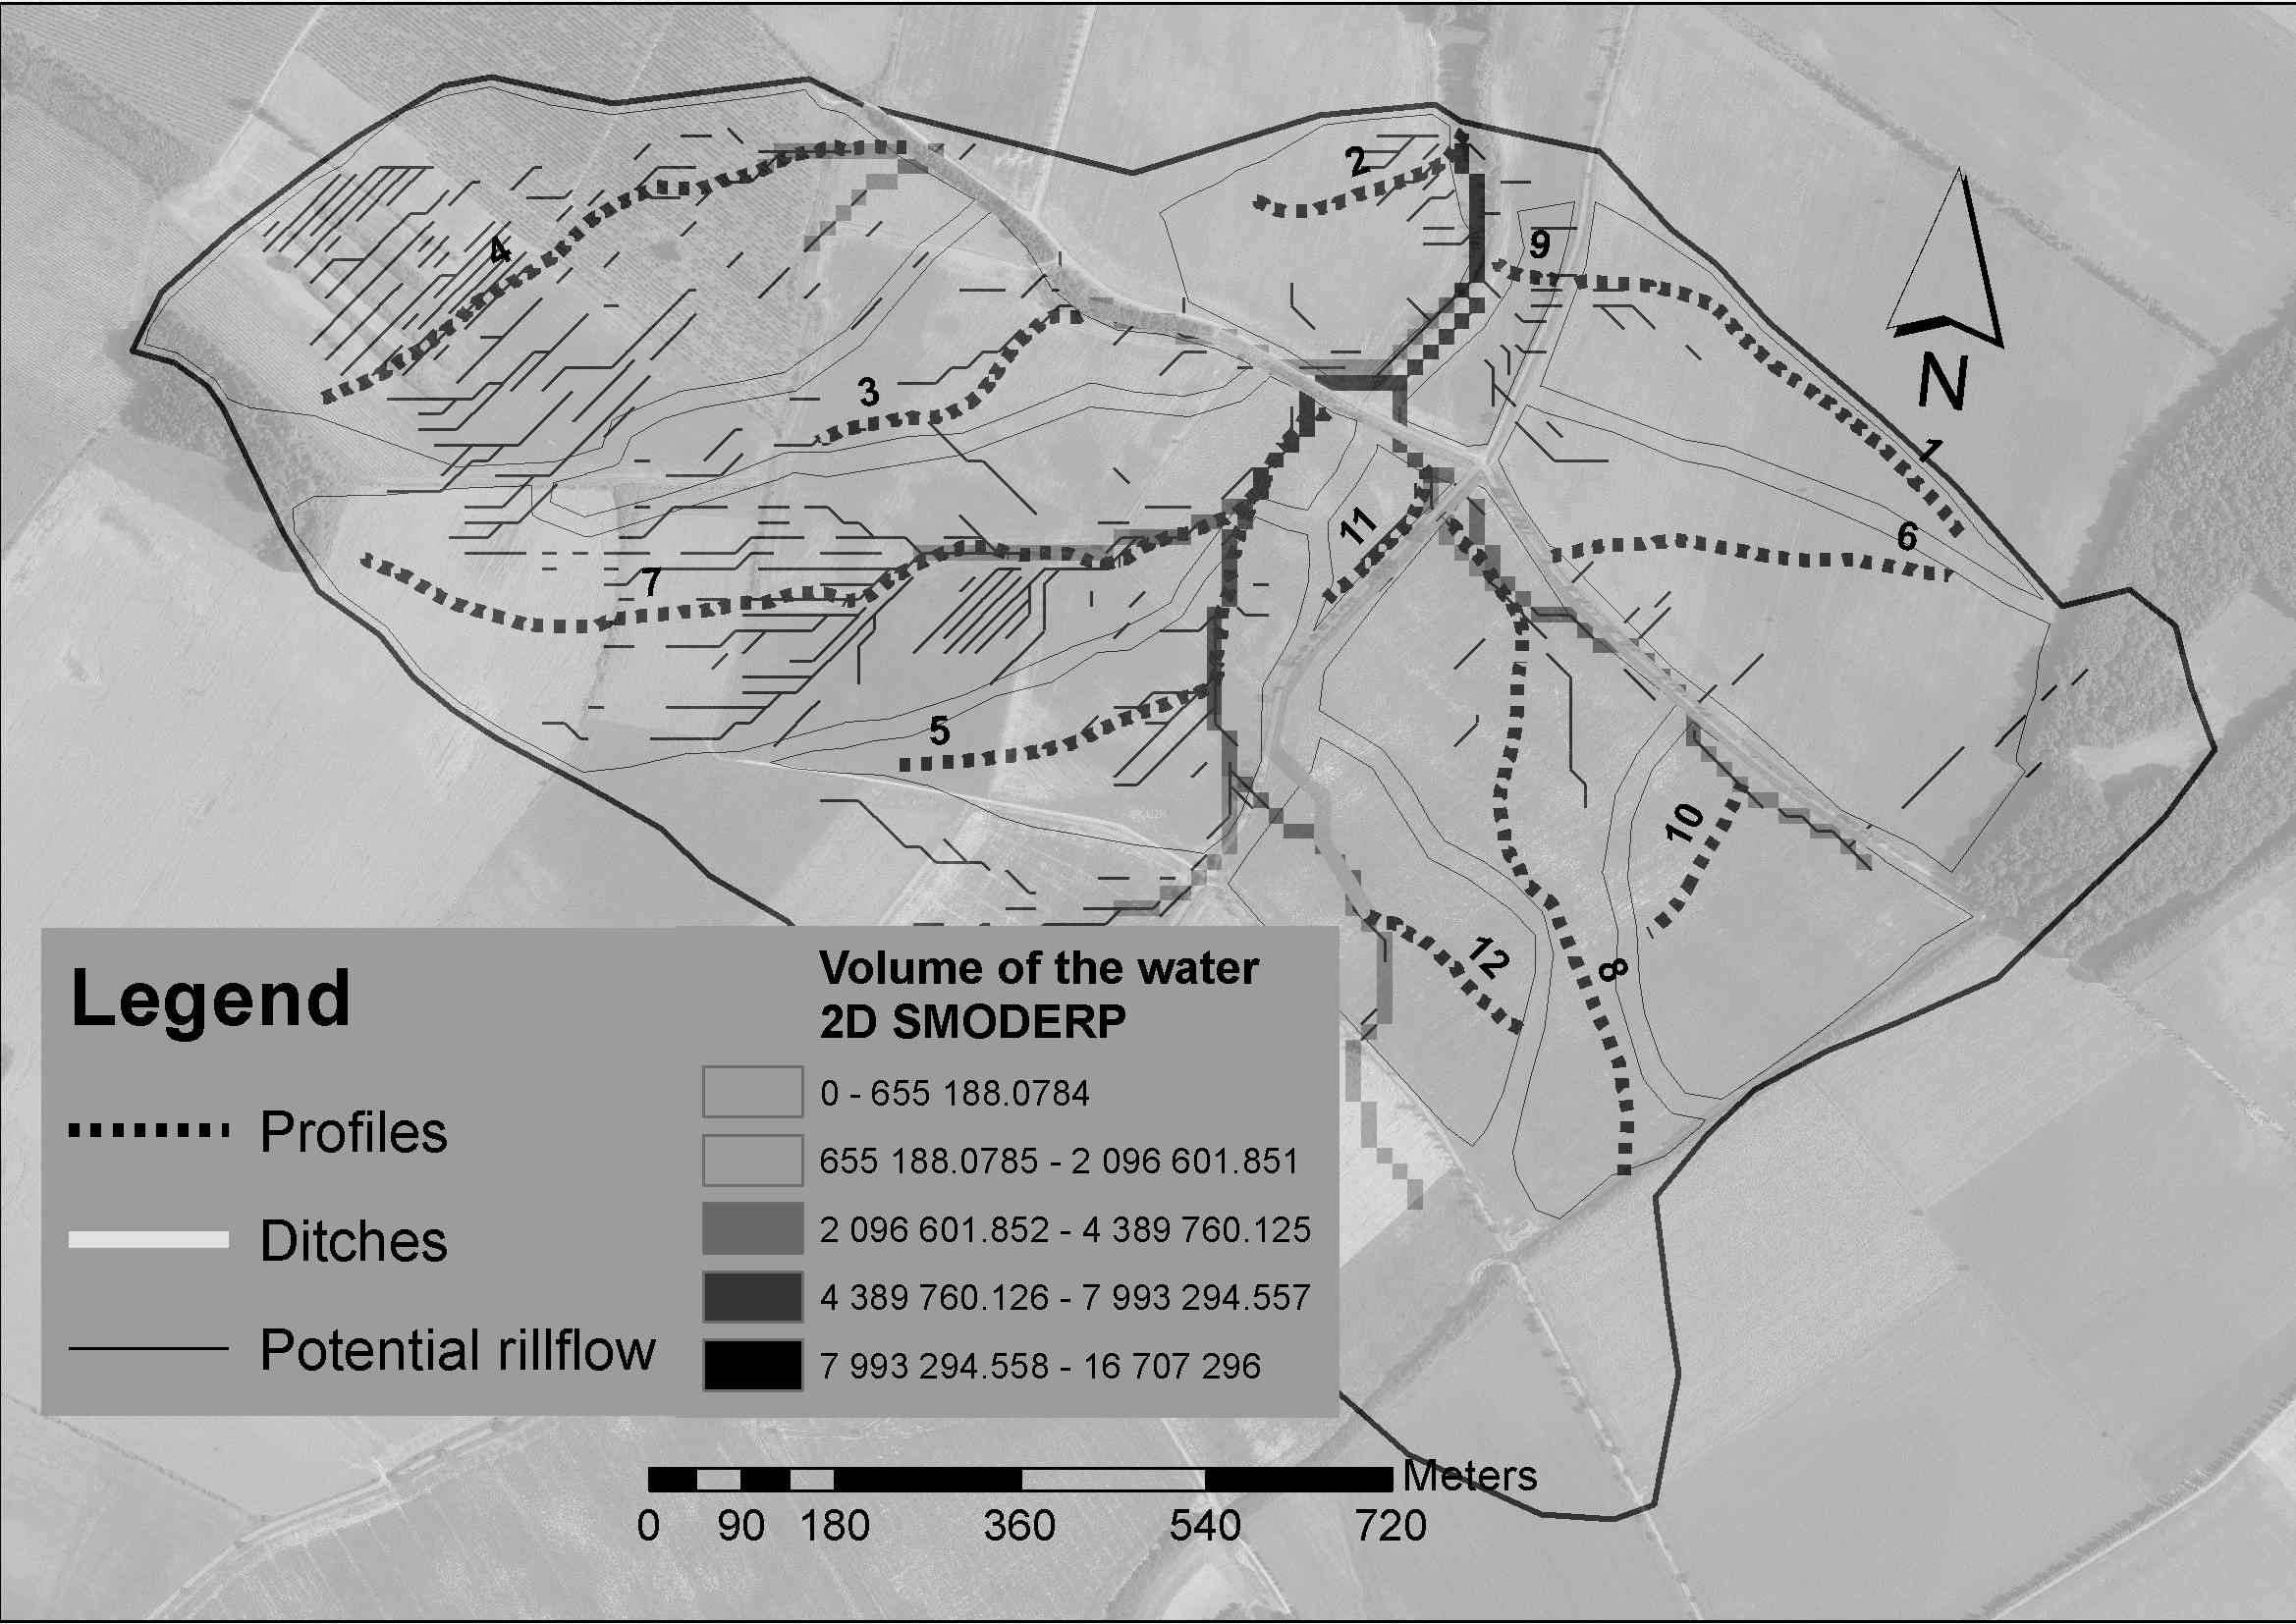
\includegraphics[width=0.8\textwidth]{img/horany_print3.jpg}
\caption{Profiles and runof concetration - Horany}
\label{fig:horany}
\end{figure}\FloatBarrier
ghg
\begin{figure}[ht!]
\renewcommand{\figurename}{Graf}
\centering
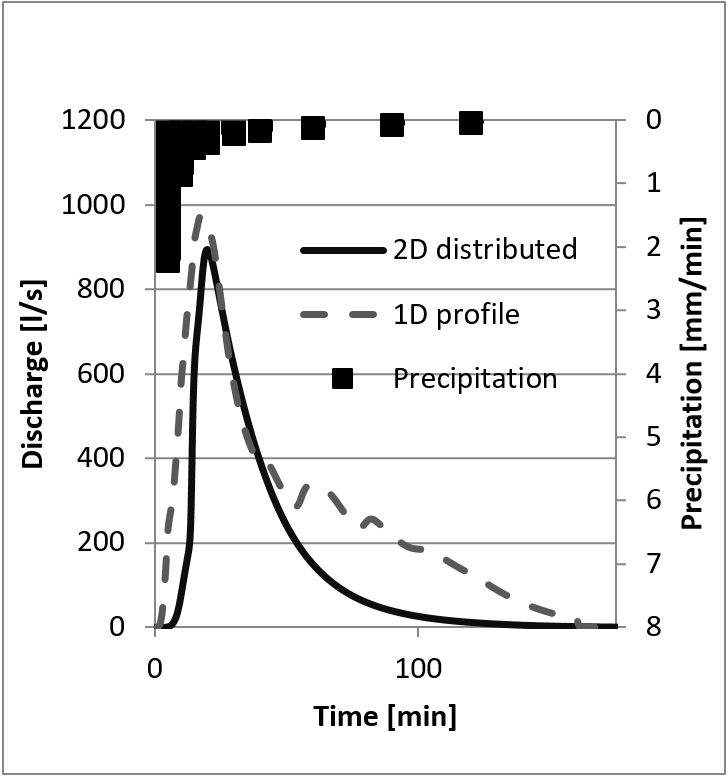
\includegraphics[width=0.8\textwidth]{graph/1D2Dhorany.png}
\caption{Hydrographs 1D and 2D Smoderp - Horany study area}
\label{graf:graf_1}
\end{figure}\FloatBarrier

The second location is formed by the independent agricultural plot situated in the Býkovický potok basin (Benešov u Prahy) with a morphologically distinctive lane of concentration runoff. Experimental measurements of erosion processes were carried out on the given plot for a considerable period of time. It is thus possible to compare the final results for the appropriate model with measured values. Six characteristic profiles were created on the given plot (size of ten acres). This number exceeds considerably the amount of profiles which were necessary for the description of the given small area. The number of profiles was appointed in order to make comparisons between 1D and 2D approaches, as well as from the reasons explaining the influence of a large number of profiles on the final characteristics. Standardized field erosion plots were installed and situated on a farmer plot in the surveyed area for monitoring the overland flow and sediment transport. The resulting cooperation between the 1D and 2D approaches was executed during the real rainstorm with measured surface runoff.

\begin{figure}[ht!]
\centering
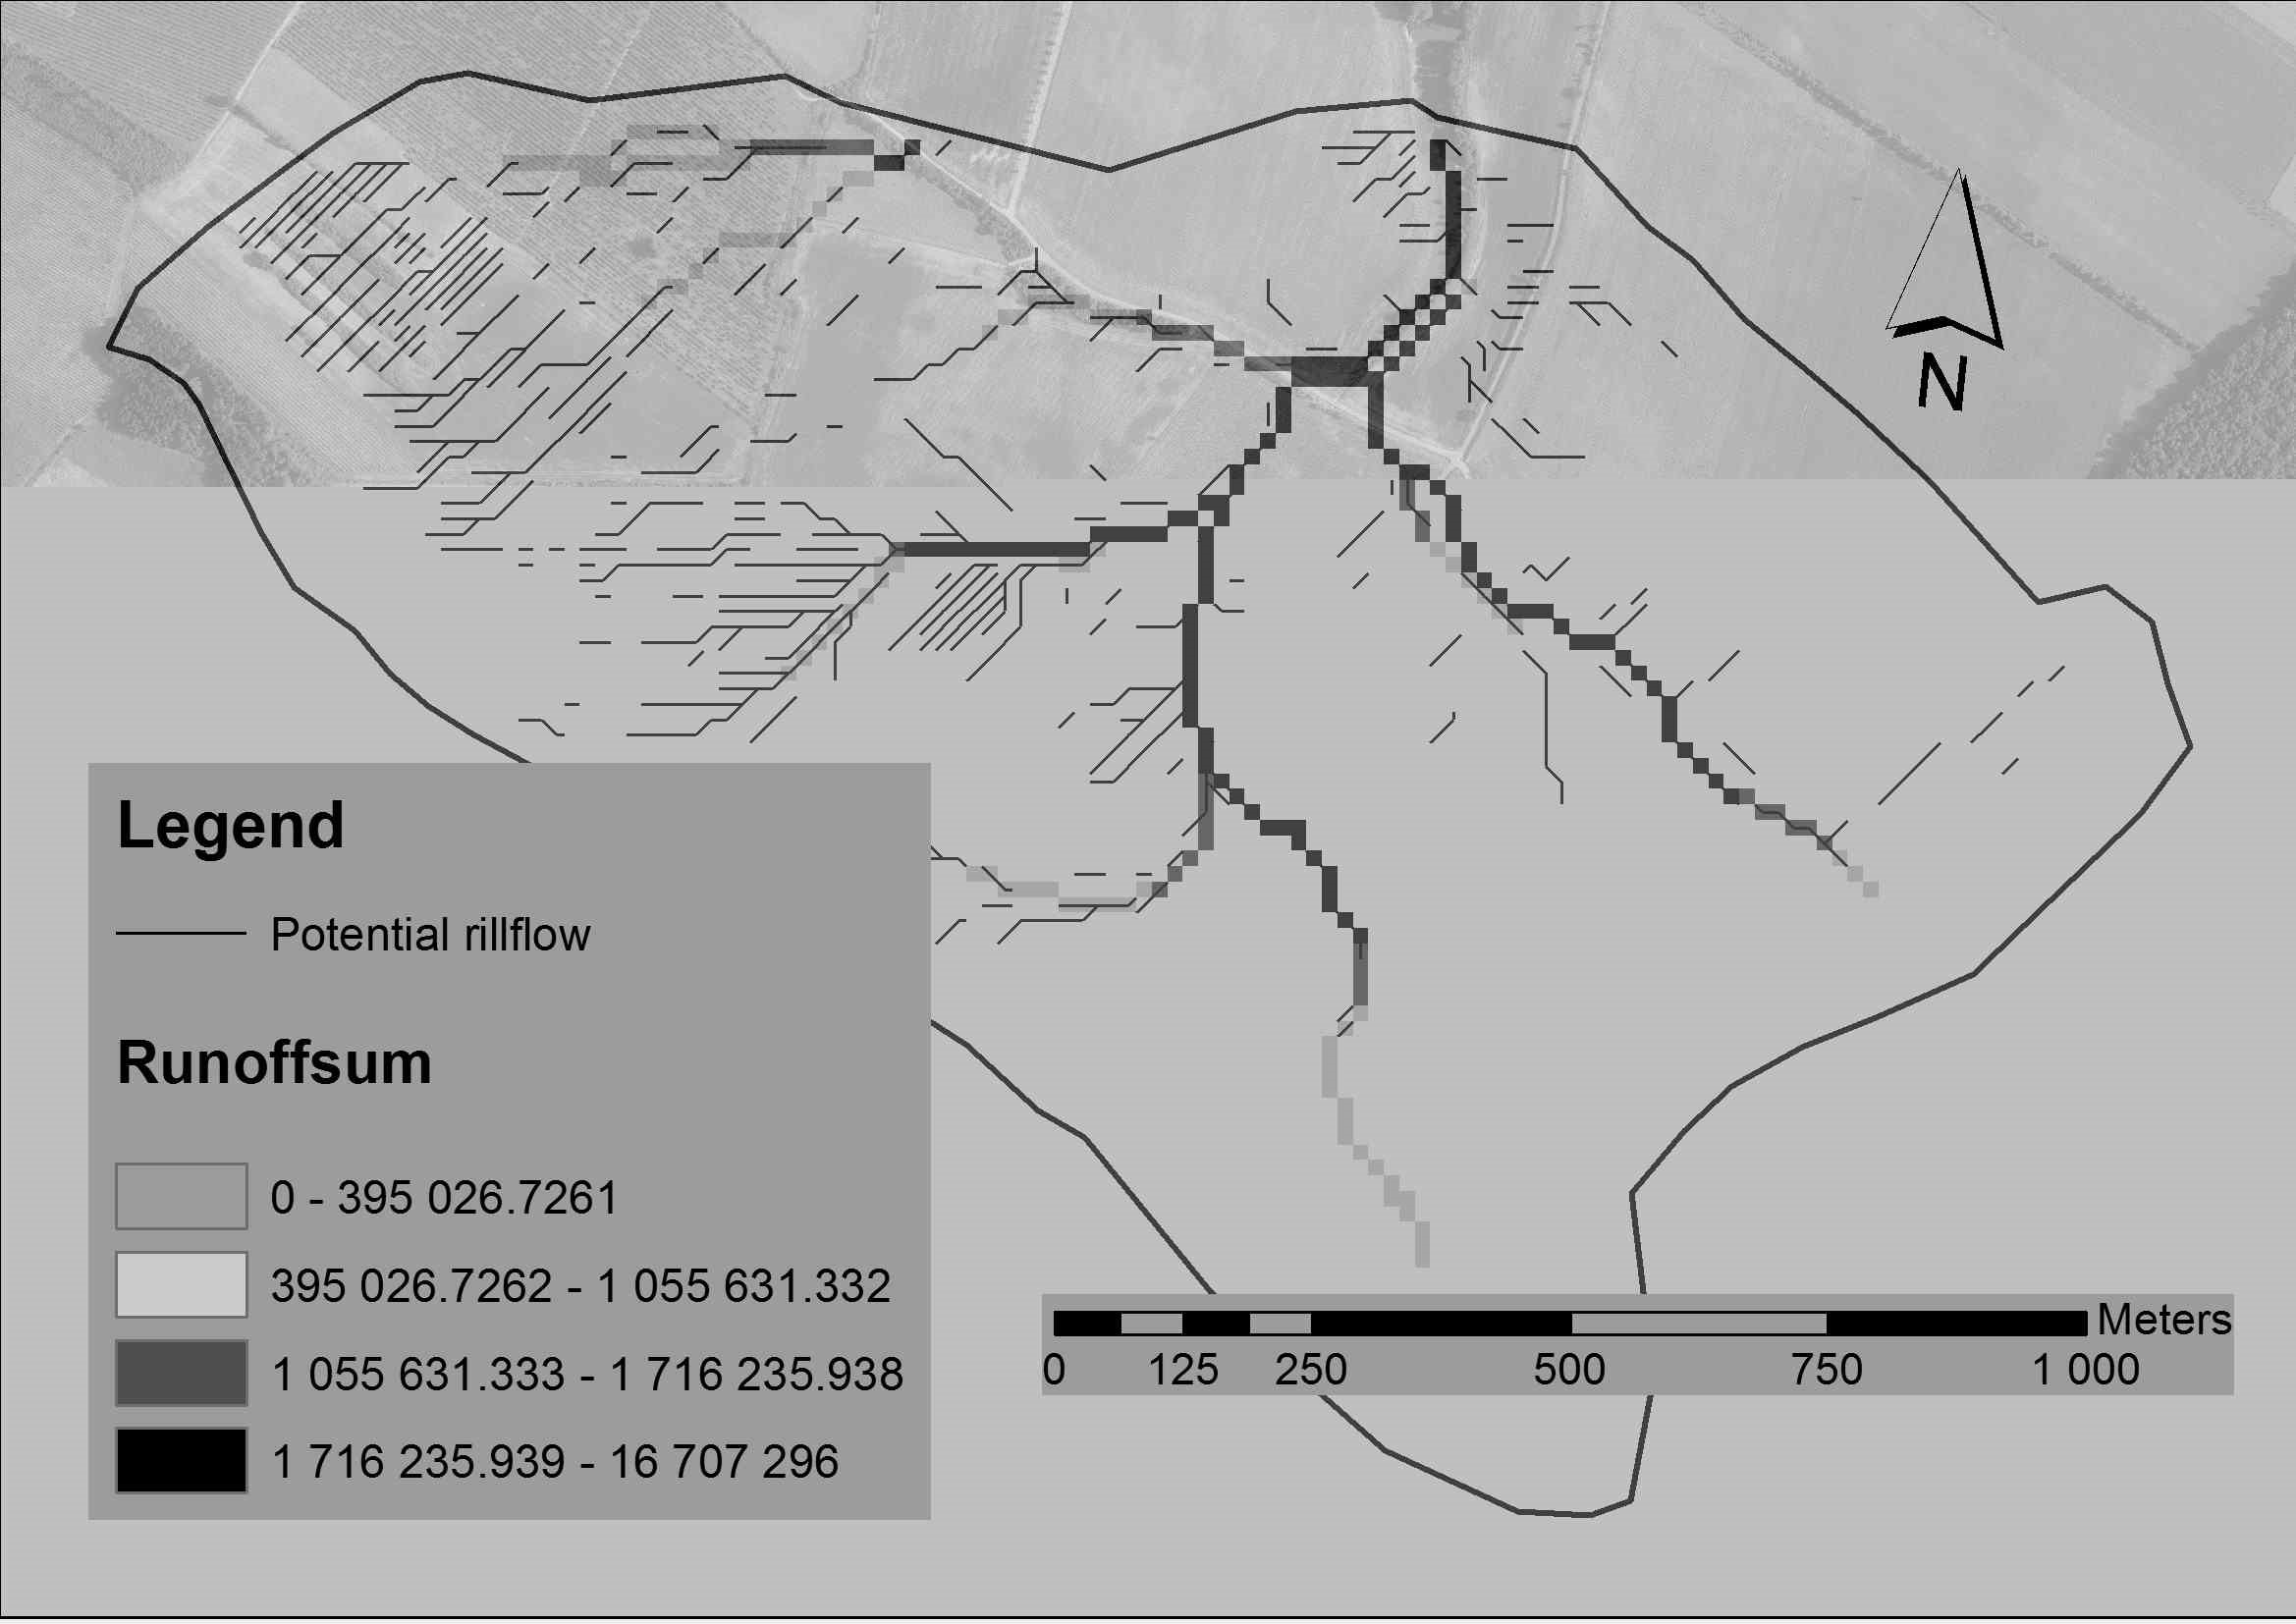
\includegraphics[width=0.8\textwidth]{img/byk.jpg}
\caption{Profiles and runof concetration - Bykovicky catchment }
\label{fig:horany}
\end{figure}\FloatBarrier

\begin{figure}[ht!]
\renewcommand{\figurename}{Graf}
\centering
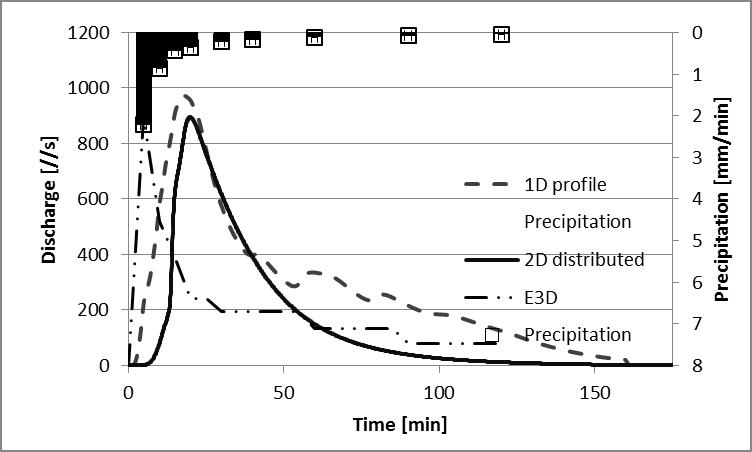
\includegraphics[width=0.8\textwidth]{graph/1D2DByk.jpg}
\caption{Hydrographs 1D and 2D Smoderp - Bykovicky catchment}
\label{graf:graf_1}
\end{figure}\FloatBarrier

The results based on hydrograph measurements taken from individual profiles in both locations were progressively added to the breach profile (outlet). In order to compare the discharge process, the values of surface level, discharge and a cell of the breach profile were extracted in the 2D model version for testing. The implementation of this process is enabled in the development environment of the particular model.